
%%%%%%%% ICML 2015 EXAMPLE LATEX SUBMISSION FILE %%%%%%%%%%%%%%%%%
%%%%%%%%%%%%%%%%%%%%%%%%%%%%%%%%%%%%%%%%%%%%%%%%%%%%%%%%%%%%%%%%%%

\documentclass{article}

\usepackage{times}
\usepackage{graphicx}
\usepackage{subfigure} 

% For citations
\usepackage{natbib}
\usepackage[utf8]{inputenc}

% For algorithms
%\usepackage{algorithm}
%\usepackage{algorithmic}
% Packages hyperref and algorithmic misbehave sometimes.  We can fix
% this with the following command.
%\newcommand{\theHalgorithm}{\arabic{algorithm}}

\usepackage{hyperref}
\usepackage{amsmath}
\usepackage{amssymb}

\def \N {\mathbb{N}}
\def \Nbr {\mathcal{N}}
\def \Q {\mathbb{Q}}
\def \F {\mathbb{F}}
\def \then {\implies &}
\def \oif {\Longleftrightarrow &\,}
\def \given {\text{Given }&}
\def \assume {\text{Assume }&}
\def \thfr {\therefore &\enskip}
\def \bij {\leftrightarrow}
\def \inj {\rightarrowtail}
\def \sur {\twoheadedrightarrow}
\def \Z {\mathbb{Z}}
\def \R {\mathbb{R}}
\def \C {\mathbb{C}}
\def \D {\mathbb{D}}
\def \H {\mathbb{H}}
\def \iff {\Longleftrightarrow}
\def \kron {\boldsymbol\delta}
\def \id {\text{id}}

\def\Tx{\textbf{x}}
\def\Ty{\textbf{y}}
\def\quotient{\mathclose{}/\mathopen{}}
\def\Tf{\textbf{f}}
\def\Th{\textbf{h}}
\def\Tg{\textbf{g}}
\def\sumn{\sum_{n=0}^\infty}
\def\limn{\lim_{n\rightarrow\infty}}
\def\prodn{\prod_{n=0}^\infty}
\DeclareMathOperator\adj{adj}

\newcommand{\stc}[1]{\widetilde{#1}}   
\newcommand{\pa}[1]{ \left({#1}\right) }
\newcommand{\set}[2]{ \left\{ #1 \,\middle|\, #2 \right\} }
\newcommand{\shift}[1]{&\quad & \text{#1}\\}
\newcommand{\lem}[1]{\text{\textbf{L.\ref{#1}}}}
\newcommand{\card}[1]{\left\vert{#1}\right\vert}
\newcommand{\Ps}[1]{\mathcal{P}\left({ #1 }\right)}
\newcommand{\colv}[1]{\begin{pmatrix} #1 \end{pmatrix}}
\newcommand{\mat}[1]{\begin{pmatrix} #1 \end{pmatrix}}
\newcommand{\detmat}[1]{\begin{vmatrix} #1 \end{vmatrix}}
\newcommand{\spanb}[1]{\text{span}\{ #1 \}}
\newcommand{\abs}[1]{\left|#1\right|}
\newcommand{\Inner}[1]{\langle #1 \rangle}
\newcommand{\Innercpy}[1]{\langle #1, #1 \rangle}
\newcommand{\conj}[1]{{\overline{#1}}}

\DeclareMathOperator{\Tr}{tr}
\DeclareMathOperator{\Dim}{dim}
\DeclareMathOperator{\Rank}{rank}
\DeclareMathOperator{\Ker}{ker}
\DeclareMathOperator{\Diam}{diam}
\DeclareMathOperator{\Diag}{diag}
\DeclareMathOperator{\Int}{int}
\DeclareMathOperator{\Clo}{clo}
\DeclareMathOperator{\sgn}{sgn}
\DeclareMathOperator{\MyRe}{Re}
\DeclareMathOperator{\MyIm}{Im}
\DeclareMathOperator{\res}{res}

% Employ the following version of the ``usepackage'' statement for
% submitting the draft version of the paper for review.  This will set
% the note in the first column to ``Under review.  Do not distribute.''
%\usepackage{icml2015} 

% Employ this version of the ``usepackage'' statement after the paper has
% been accepted, when creating the final version.  This will set the
% note in the first column to ``Proceedings of the...''
\usepackage[accepted]{icml2015}


% The \icmltitle you define below is probably too long as a header.
% Therefore, a short form for the running title is supplied here:
\icmltitlerunning{Commodities Forecasting with GDELT}

\begin{document} 

\twocolumn[
\icmltitle{Commodities Forecasting from Non-Financial World News from GDELT}

% It is OKAY to include author information, even for blind
% submissions: the style file will automatically remove it for you
% unless you've provided the [accepted] option to the icml2015
% package.
\icmlauthor{Vladimir Feinberg}{vyf@princeton.edu}
\icmladdress{Princeton University}
\icmlauthor{Daway Chou-Ren}{dchouren@princeton.edu}
\icmladdress{Princeton University}

% You may provide any keywords that you 
% find helpful for describing your paper; these are used to populate 
% the "keywords" metadata in the PDF but will not be shown in the document
\icmlkeywords{GDELT, commodities, finance, forecasting, clustering, machine learning, ICML}

\vskip 0.3in
]

\begin{abstract} 

%TODO fill in abstract.

\end{abstract} 

%TODO review below
% Submissions must be in PDF.
% The maximum paper length is \textbf{8 pages excluding references, and 10 pages including references} (pages 9 and 10 must contain only references).
% Do \textbf{not include author information or acknowledgments} in your initial submission. 
% Your paper should be in \textbf{10 point Times font}.
% Make sure your PDF file only uses Type-1 fonts.
% Place figure captions {\em under} the figure (and omit titles from inside the graphic file itself).  Place table captions {\em over} the table.
% References must include page numbers whenever possible and be as complete as possible.  Place multiple citations in chronological order.  
% Do not alter the style template; in particular, do not compress the paper format by reducing the vertical spaces.

\section{Introduction}
 
All submissions must follow the same format to ensure the printer can
reproduce them without problems and to let readers more easily find
the information that they desire.

Tables contain textual material that can be typeset, as contrasted 
with figures, which contain graphical material that must be drawn. 
Specify the contents of each row and column in the table's topmost
row. Again, you may float tables to a column's top or bottom, and set
wide tables across both columns, but place two-column tables at the
top or bottom of the page.

\section{Motivating Analysis}


\subsection{GDELT Dataset}

\subsubsection{Sparsity in GDELT}

The space of news events spanned by all columns in GDELT is much larger than the subspace we expect news to lie on. Confirming these suspicions is important because it would indicate a need to reduce the dimensionality of the data set we are working with.

Classical dimensionality reduction was not tractable to apply to a dataset of this size - the highly categorical nature of the dataset results in a large dimensional expansion when preparing numeric inputs to the algorithms. A fast neighborhood-embedding method, tSNE, relies only on a metric between data points. Unfortunately, its runtime and space consumption grows exponentially in the reduced dimension, and extremely small dimensions yielded poor results \yrcite{van2008visualizing}.

However, it is critical to observe some sparsity in the GDELT space to confirm our clustering-based approach.

We guessed that there are likely to be at least two modes of low-dimensional interactions in the data: (1) that actors only interact within small cliques and (2) that each actors to small sets of events. We conducted this initial analysis on a random sample of days before August 2015 to avoid making conclusions that overfit the test data.

\begin{figure}[ht]
\vskip 0.2in
\begin{center}
%\centerline{\includegraphics[width=\columnwidth]{}}
\caption{
BOX WHISKER HERE. DESCRIBE 5 FIGURE SUMMARIES, OUTLIER
}
\end{center}
\vskip -0.2in
\label{fig:events-per-actor}
\end{figure} 


\begin{figure}[ht]
\vskip 0.2in
\begin{center}
%\centerline{\includegraphics[width=\columnwidth]{}}
\caption{TODO: take another random sample, histogram it. Describe summary stats. number of Distinct events per actor.}
\end{center}
\vskip -0.2in
\label{fig:events-per-actor}
\end{figure} 


As Figure \ref{fig:actors-per-actor} demonstrates, actor count is heavily skewed distribution. This gives us confidence in (1) for the sampled days. We conduct a similar inspection for the number of unique CAMEO coded events per actor in Figure \ref{fig:events-per-actor}:

\begin{figure}[ht]
\vskip 0.2in
\begin{center}
%\centerline{\includegraphics[width=\columnwidth]{}}
\caption{TODO: take another random sample, histogram it. Describe summary stats. number of Distinct events per actor.}
\end{center}
\vskip -0.2in
\label{fig:events-per-actor}
\end{figure} 

In addition to more compact data representation and reduction of noise, dimensionality reduction has several other attractive features for this dataset. First, it enables us to work in a continuous space of reduced-dimension tuples of real values, which is much easier for model generation than partially categorical variables. Secondly, the large volume of the data set implies that any size reductions that can be gained will result in more manageable data pipelines

\subsection{Bloomberg Commodity Prices}

up and down spikes

normally distributed about 0

\section{Related Work}

\section{Methods}

\section{Evaluation}

\section{Results}

%TODO remember to add runtime info

\subsection{Software and Data}

All code used is available at \hyperref[https://github.com/vlad17/COS513-Finance]{''https://github.com/vlad17/COS513-Finance''}. GDELT provides free access to its database as well: \hyperref[http://data.gdeltproject.org/events/index.html]{''http://data.gdeltproject.org/events/index.html''}.

%TODO commodities data
%\footnote{Example footnote should have full sentences.}

% Acknowledgements should only appear in the accepted version. 
% \section*{Acknowledgments} 

% In the unusual situation where you want a paper to appear in the
% references without citing it in the main text, use \nocite
% \nocite{langley00}

\bibliography{biblio}
\bibliographystyle{icml2015}

\end{document} 

%\begin{figure}[ht]
%\vskip 0.2in
%\begin{center}
%\centerline{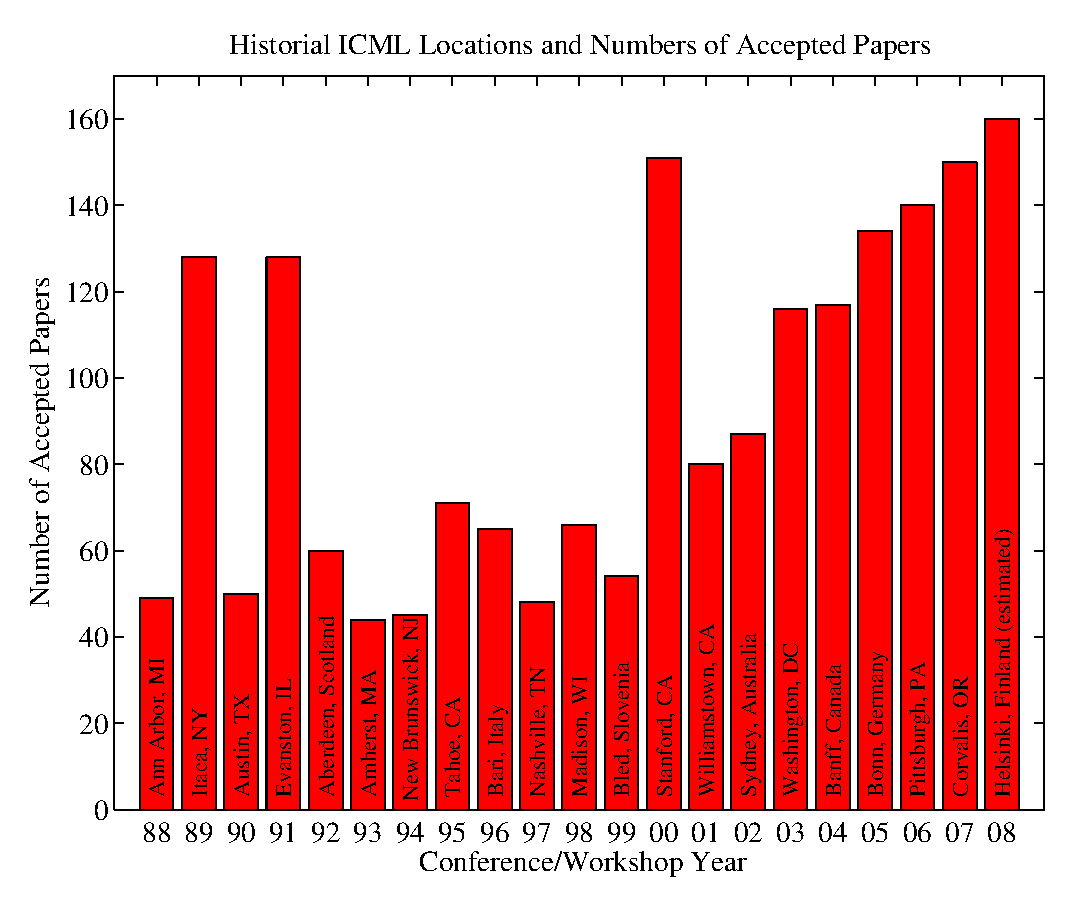
\includegraphics[width=\columnwidth]{icml_numpapers}}
%\caption{Historical locations and number of accepted papers for International
%  Machine Learning Conferences (ICML 1993 -- ICML 2008) and
%  International Workshops on Machine Learning (ML 1988 -- ML
%  1992). At the time this figure was produced, the number of
%  accepted papers for ICML 2008 was unknown and instead estimated.}
%\label{icml-historical}
%\end{center}
%\vskip -0.2in
%\end{figure} 

%Citations within the text should include the authors' last names and
%year. If the authors' names are included in the sentence, place only
%the year in parentheses, for example when referencing Arthur Samuel's
%pioneering work \yrcite{Samuel59}. Otherwise place the entire
%reference in parentheses with the authors and year separated by a
%comma \cite{Samuel59}. List multiple references separated by
%semicolons \cite{kearns89,Samuel59,mitchell80}. Use the `et~al.'
%construct only for citations with three or more authors or after
%listing all authors to a publication in an earlier reference \cite{MachineLearningI}.

% EXAMPLE TABLE
%\begin{table}[t]
%\caption{Classification accuracies for naive Bayes and flexible 
%Bayes on various data sets.}
%\label{sample-table}
%\vskip 0.15in
%\begin{center}
%\begin{small}
%\begin{sc}
%\begin{tabular}{lcccr}
%\hline
%\abovespace\belowspace
%Data set & Naive & Flexible & Better? \\
%\hline
%\abovespace
%Breast    & 95.9$\pm$ 0.2& 96.7$\pm$ 0.2& $\surd$ \\
%Cleveland & 83.3$\pm$ 0.6& 80.0$\pm$ 0.6& $\times$\\
%Glass2    & 61.9$\pm$ 1.4& 83.8$\pm$ 0.7& $\surd$ \\
%Credit    & 74.8$\pm$ 0.5& 78.3$\pm$ 0.6&         \\
%Horse     & 73.3$\pm$ 0.9& 69.7$\pm$ 1.0& $\times$\\
%Meta      & 67.1$\pm$ 0.6& 76.5$\pm$ 0.5& $\surd$ \\
%Pima      & 75.1$\pm$ 0.6& 73.9$\pm$ 0.5&         \\
%\belowspace
%Vehicle   & 44.9$\pm$ 0.6& 61.5$\pm$ 0.4& $\surd$ \\
%\hline
%\end{tabular}
%\end{sc}
%\end{small}
%\end{center}
%\vskip -0.1in
%\end{table}